\chapter{Workflow (as is) na notação BPMN}\label{sec:3}

Workflow (as is), na notação BPMN (Business Process Model and Notation), é uma representação gráfica de um processo de negócio conforme ele é atualmente executado. Ele descreve as atividades, decisões, eventos e fluxos de informações que ocorrem durante a realização de uma tarefa ou conjunto de tarefas dentro de uma organização. O objetivo do Workflow (as is) na notação BPMN é fornecer uma visão clara e detalhada do processo existente, destacando os pontos de entrada, saída, decisões e interações entre os elementos do processo. Isso permite uma compreensão completa e precisa do fluxo de trabalho atual, facilitando a identificação de áreas de melhoria e otimização.


Na Figura \ref{fig:11} , é apresentado o BPMP (as is) do gerenciamento de agendamento, onde mostra os processos de como os clientes fazem os agendamentos de suas consultas atualmente.

Na Figura \ref{fig:12}, é apresentado o BPMP (as is) do gerenciamento de compromissos, onde mostra os processos de como o advogado da MR Telles atualmente gerencia seus processos.

Na Figura \ref{fig:13}, é apresentado o BPMP (as is) do gerenciamento de processos, onde os clientes procuram o advogado para pedir informações sobre seus casos, tirar dúvidas e esclarecer qualquer mal-entendido durante o processo.

Na Figura \ref{fig:14}, é apresentado o BPMP (as is) do gerenciamento financeiro, onde mostra os processos de como o advogado da MR Telles gerencia suas demandas financeiras nas organizações e verifica seus valores.

Na Figura \ref{fig:15}, é apresentado o BPMP (as is) do gerenciamento de pagamento, onde mostra os processos de como o advogado da MR Telles gerencia suas demandas financeiras nas organizações, confere com o cliente, aplica desconto caso tenha sido negociado e, após isso, valida para passar ao cliente.


\begin{figure}
    \centering
    \caption{Agendamento-(as is)}
    \label{fig:11}
    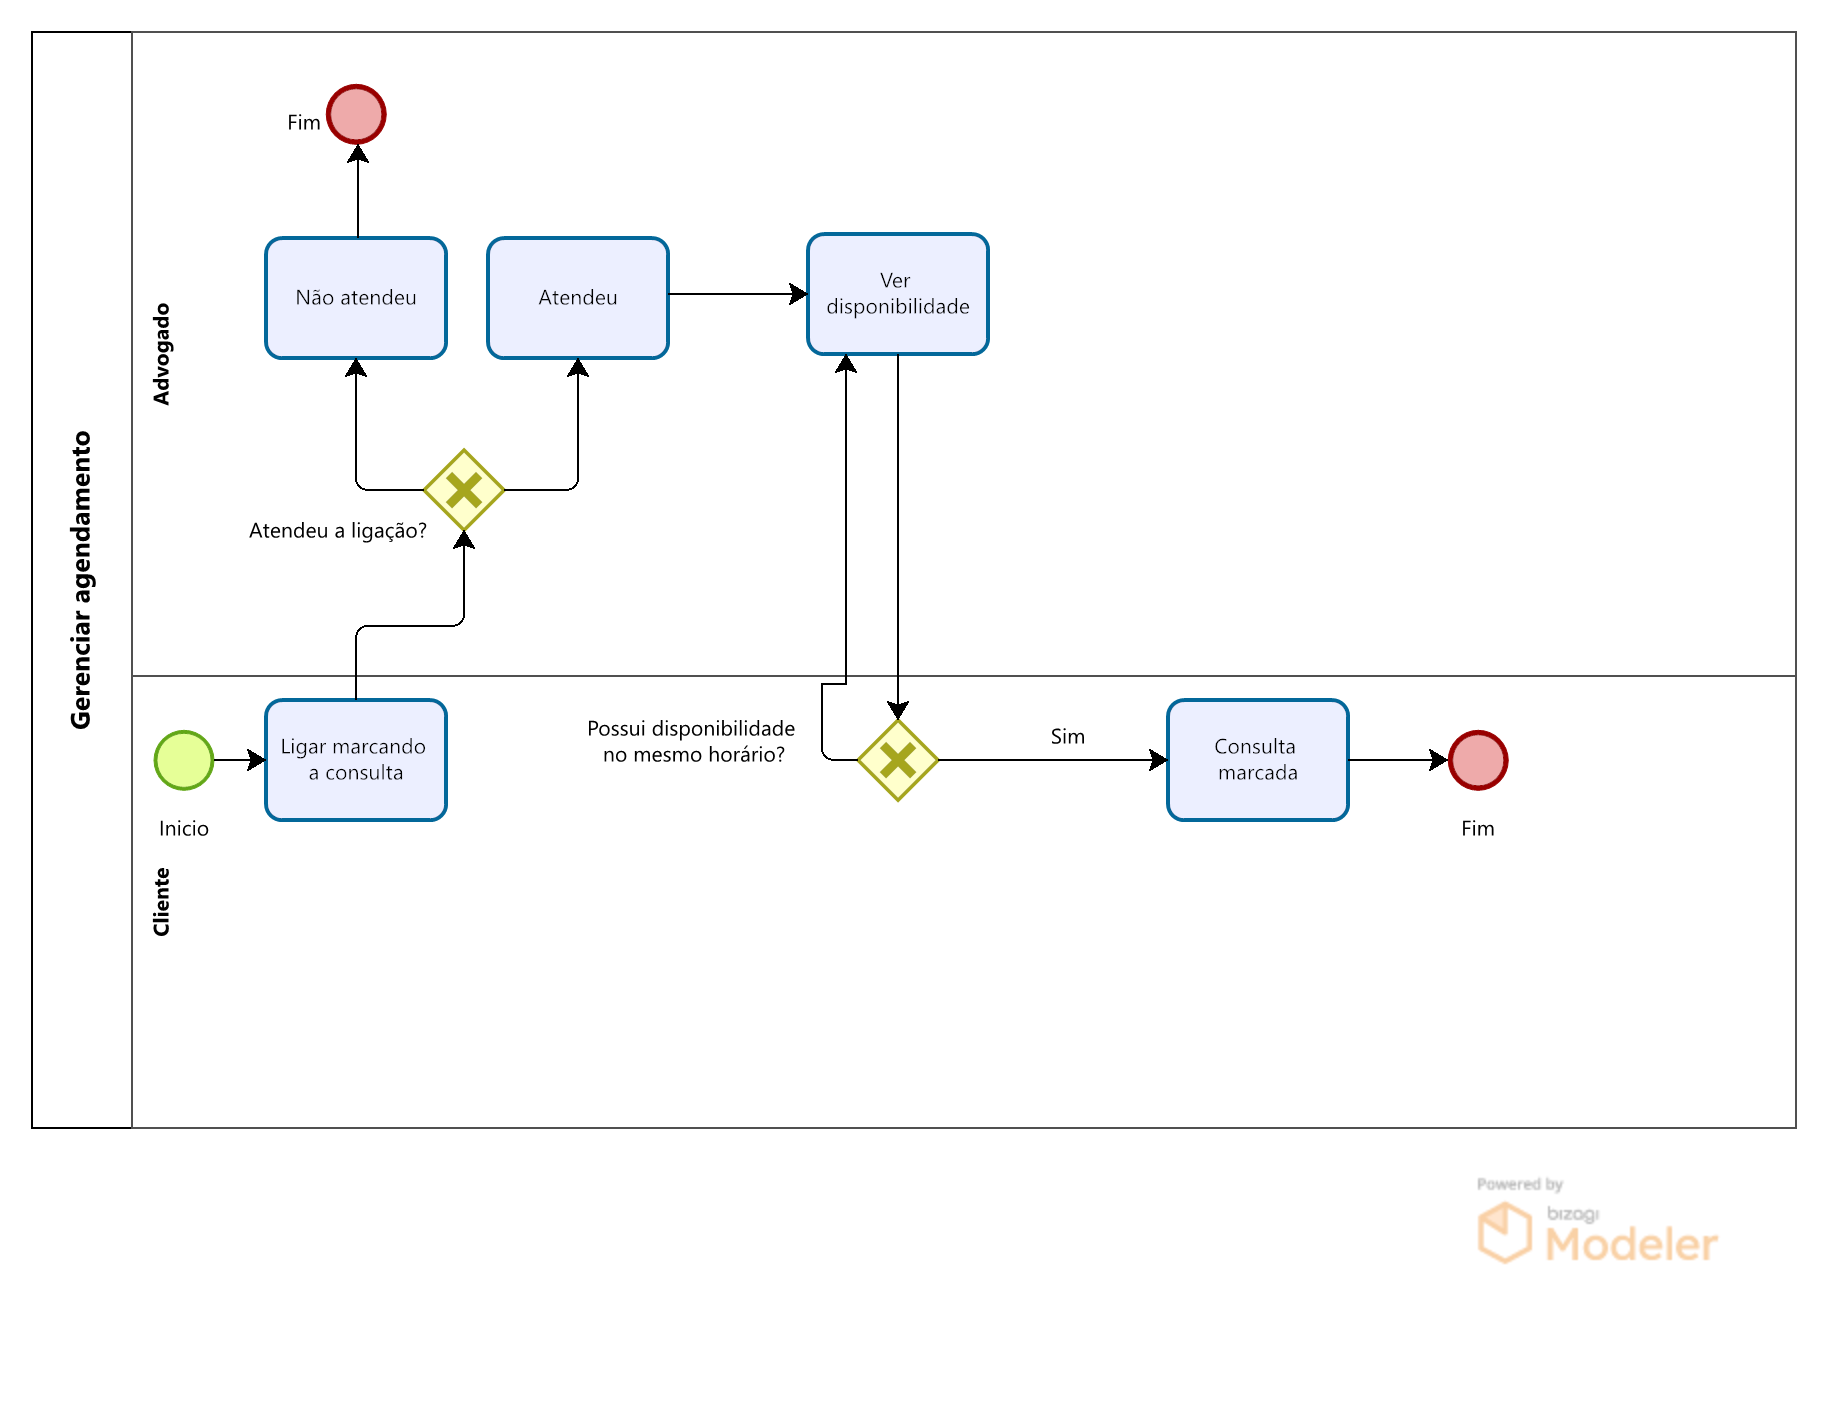
\includegraphics[width=0.8\linewidth]{imagens/BPMN/gerenciarAgendamento.png}
\end{figure}

\begin{figure}
    \centering
    \caption{Compromisso-(as is)}
    \label{fig:12}
    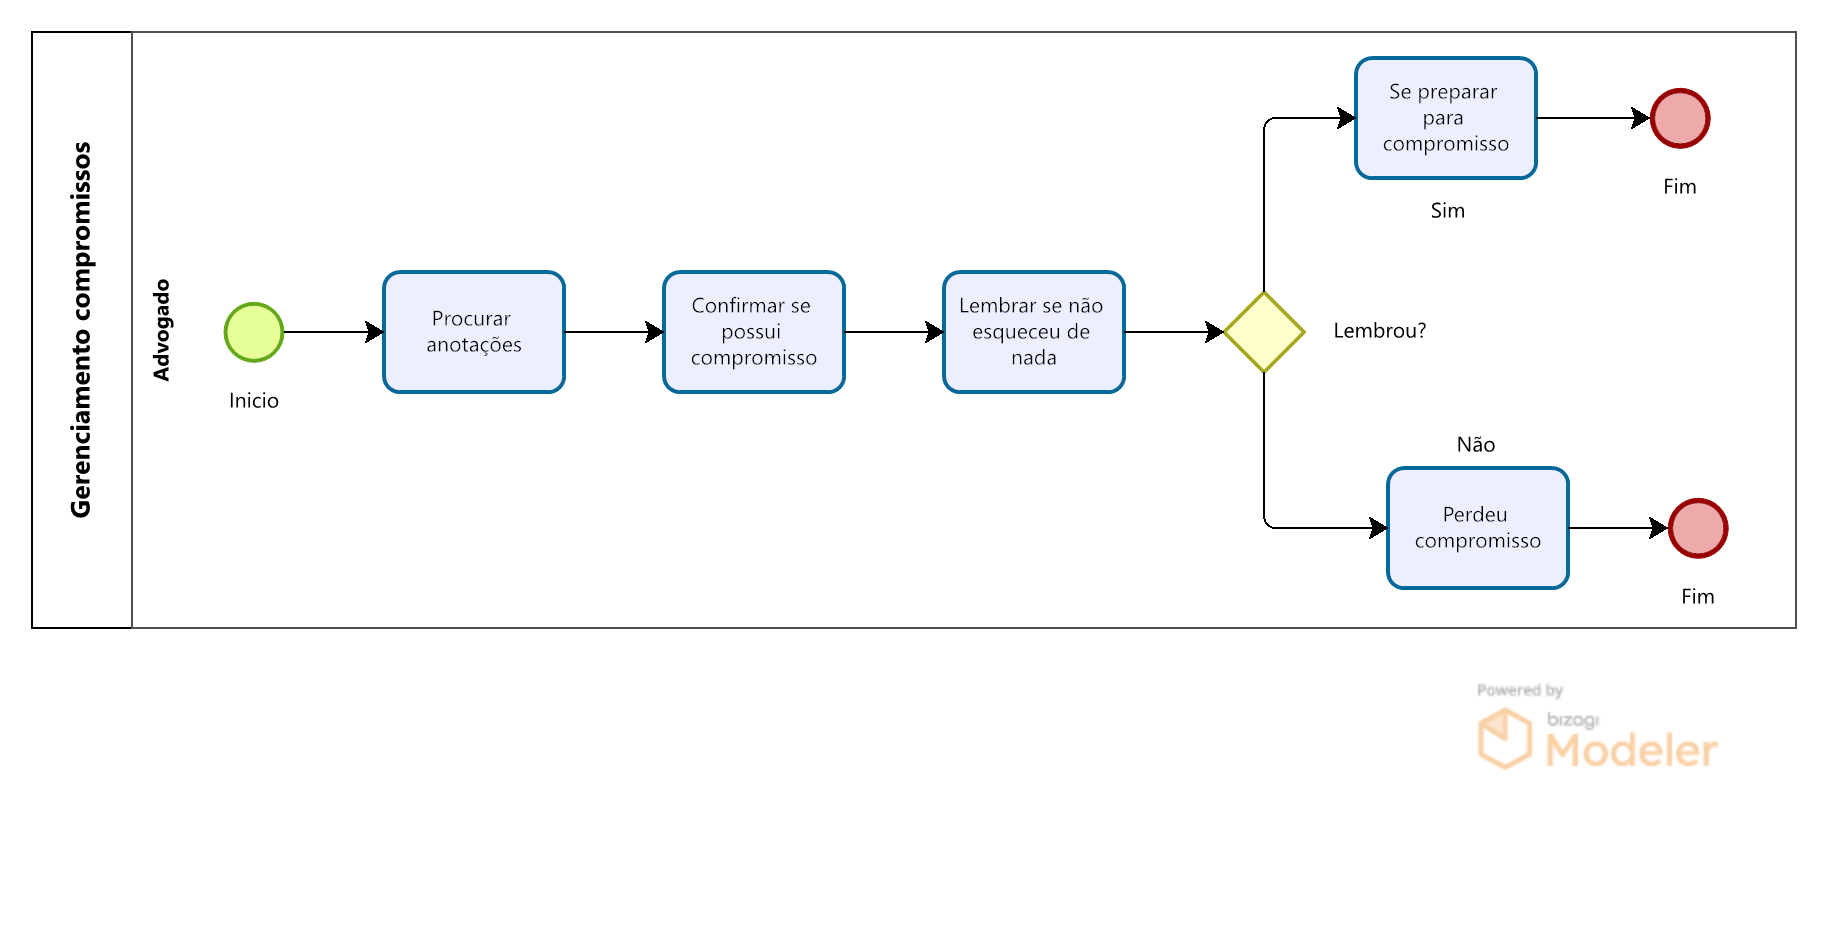
\includegraphics[width=0.8\linewidth]{imagens/BPMN/gerenciarCompromisso.png}
\end{figure}

\begin{figure}
    \centering
    \caption{Processos-(as is)}
    \label{fig:13}
    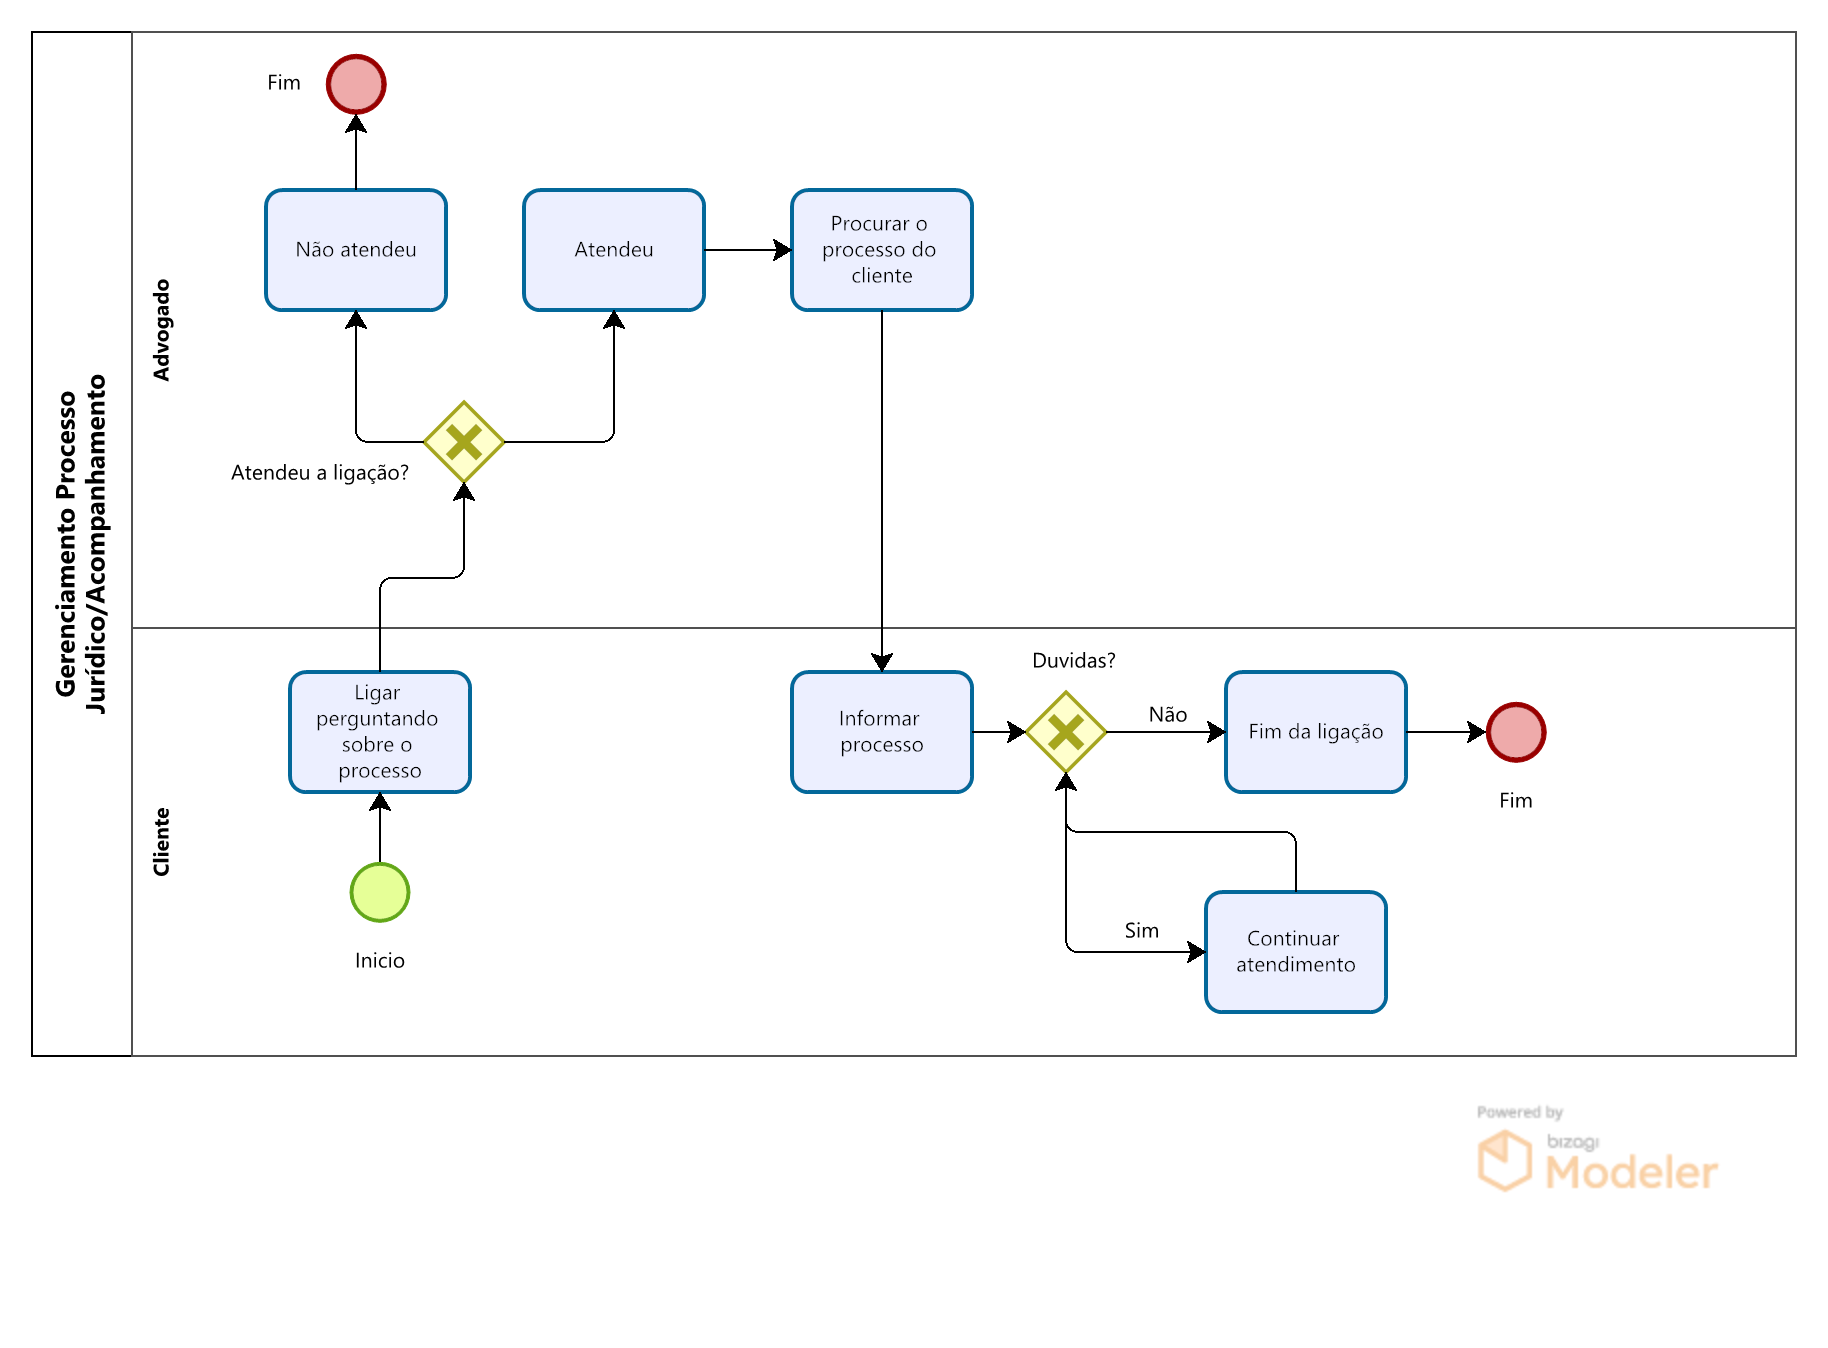
\includegraphics[width=0.8\linewidth]{imagens/BPMN/gerenciarProcesso.png}
\end{figure}

\begin{figure}
    \centering
    \caption{Financeiro-(as is)}
    \label{fig:14}
    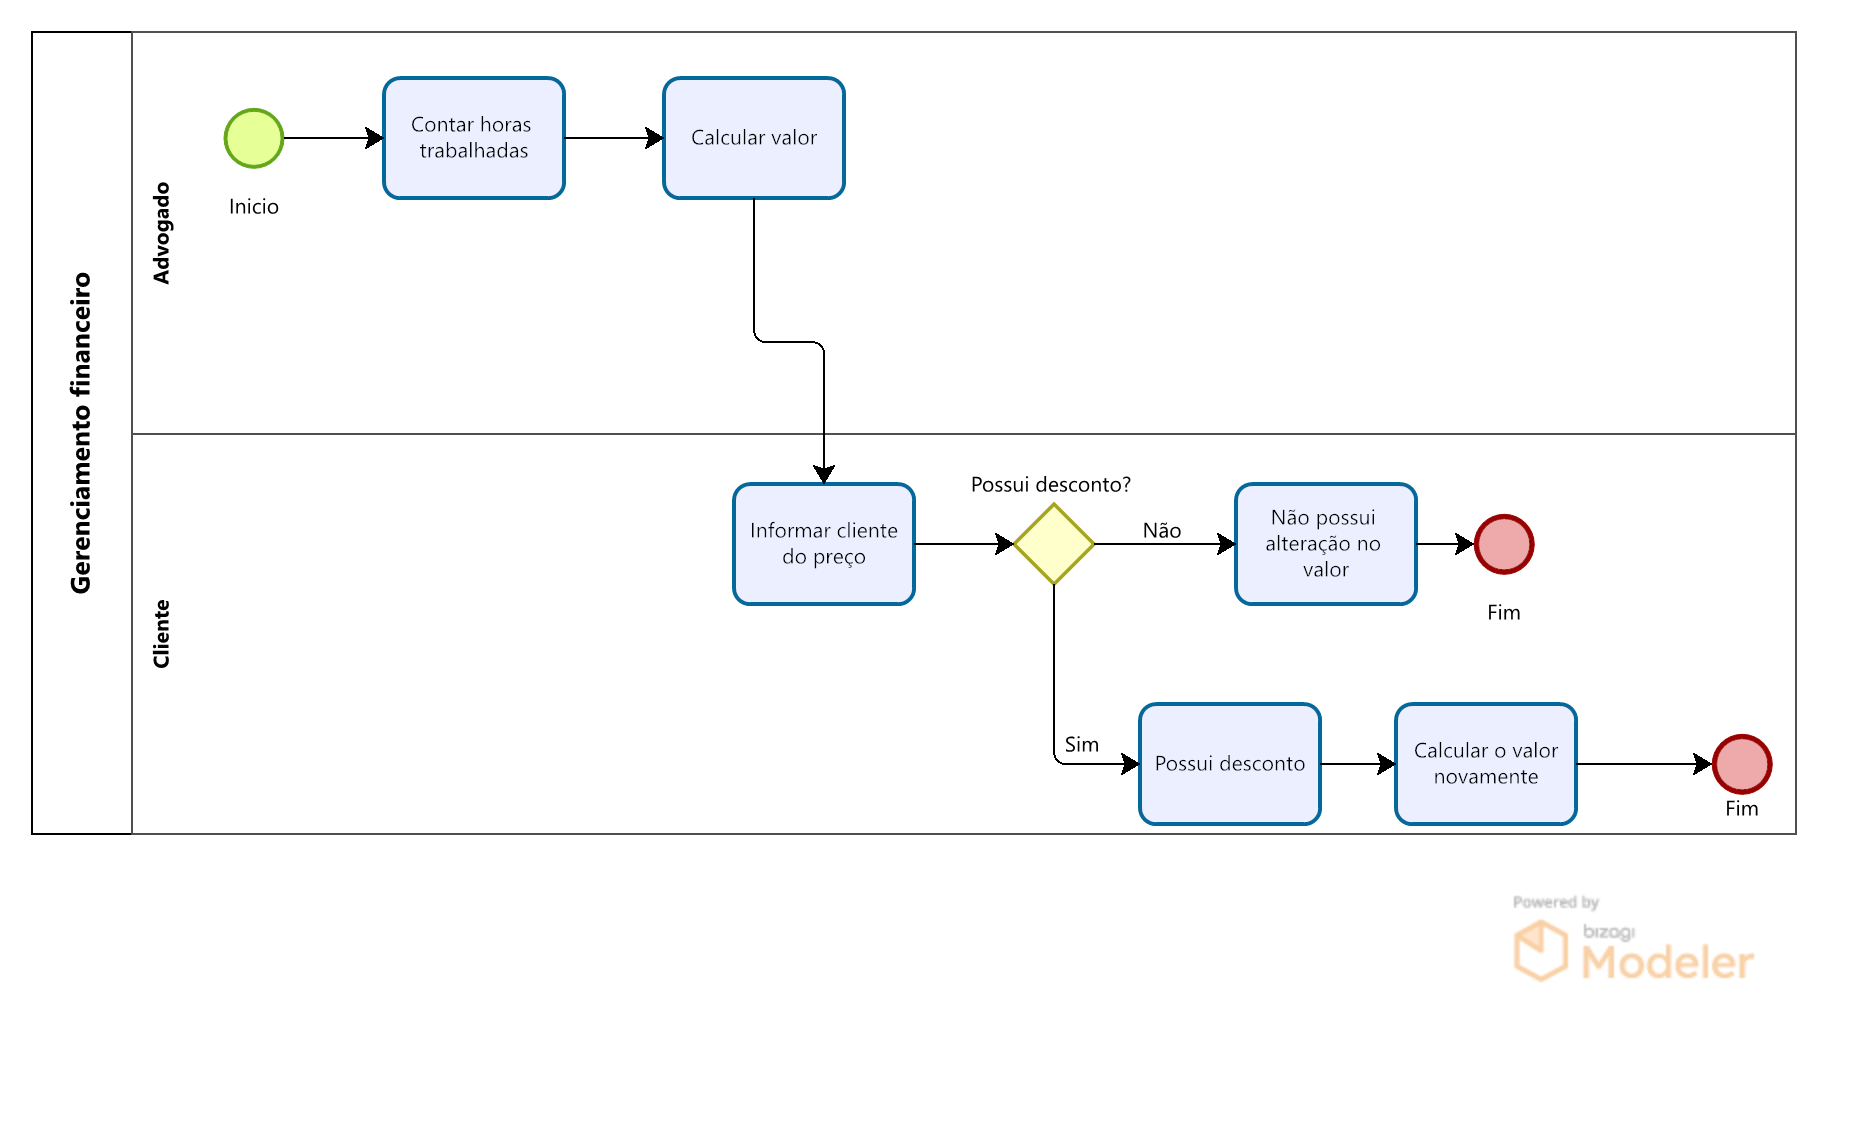
\includegraphics[width=0.8\linewidth]{imagens/BPMN/gerenciarFinanceiro.png}
\end{figure}

\begin{figure}
    \centering
    \caption{Pagamento-(as is)}
    \label{fig:15}
    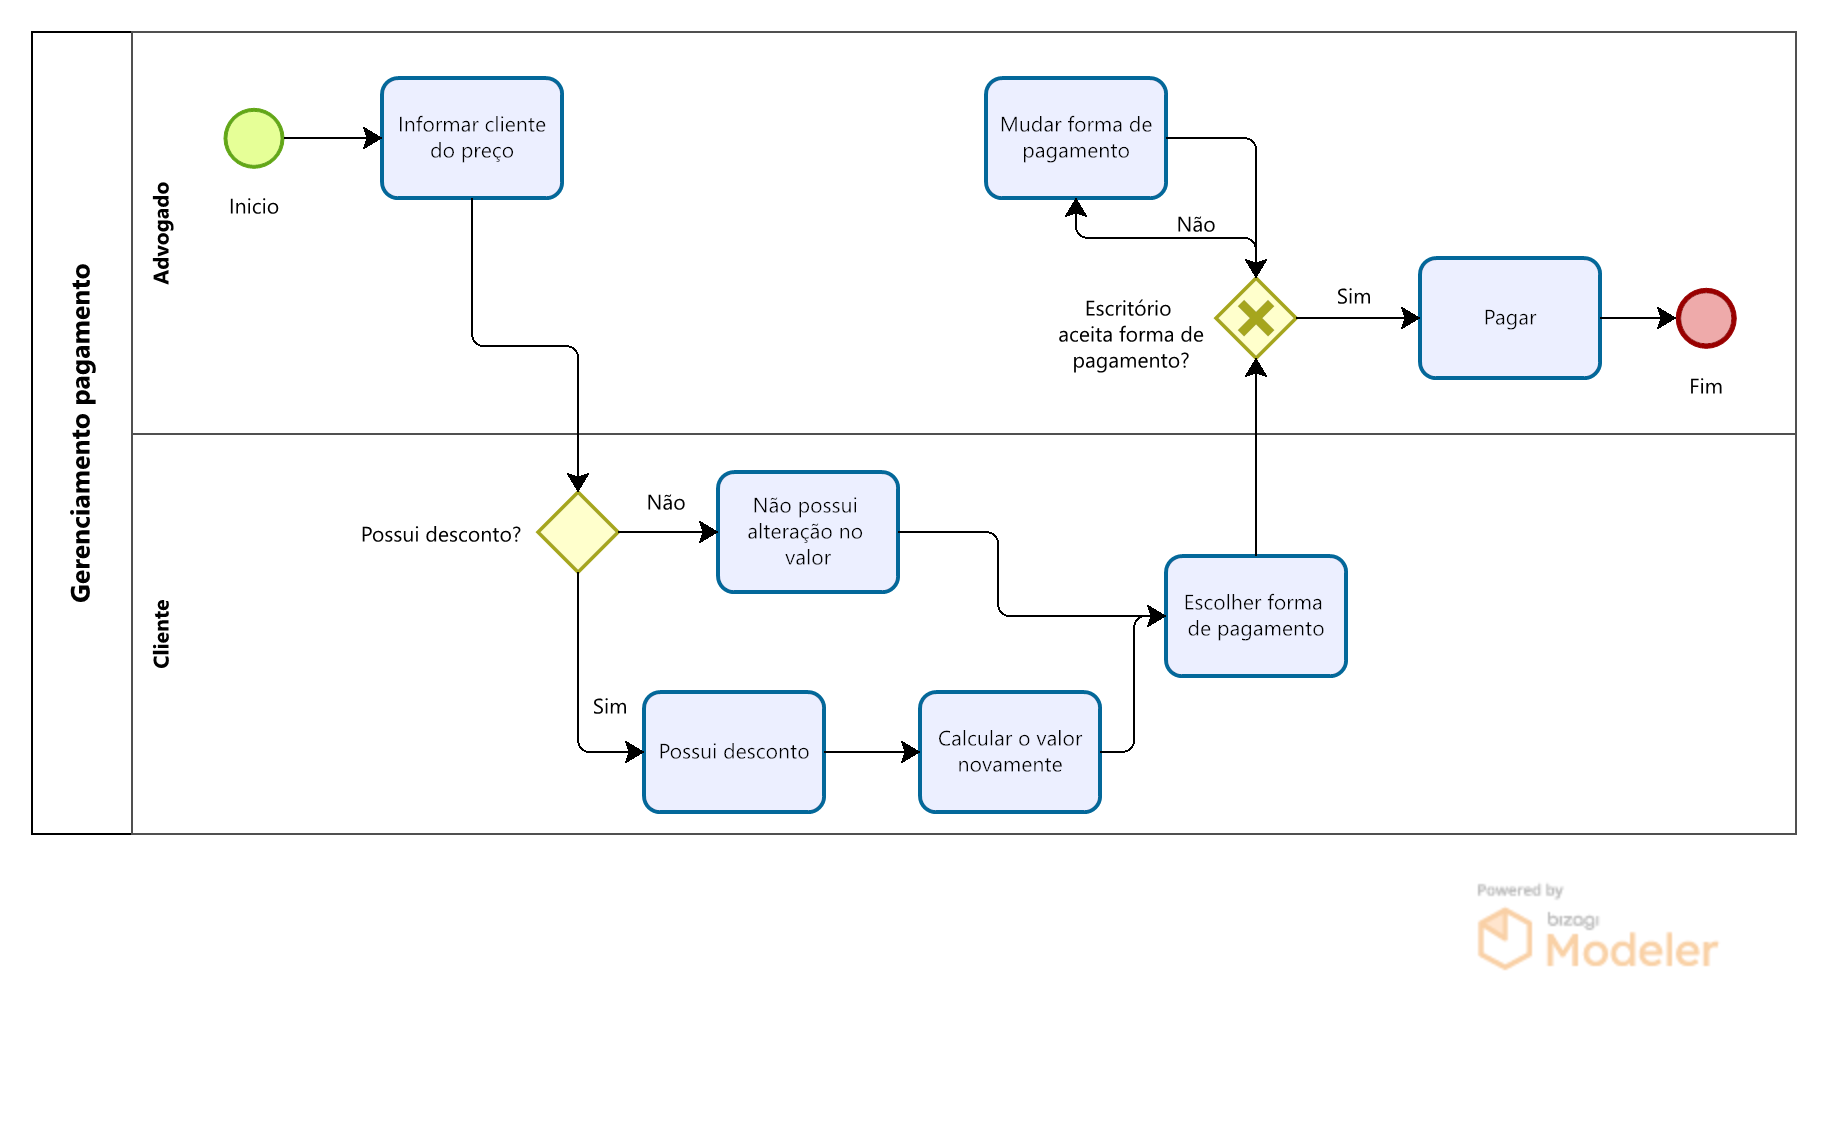
\includegraphics[width=0.8\linewidth]{imagens/BPMN/gerenciarPagamento.png}
\end{figure}
